\documentclass{book}
\usepackage{listings}
\usepackage{hyperref}
\usepackage{verbatim}
\usepackage{amsmath}
\usepackage[backend=bibtex, sorting=none, style=numeric-comp, defernumbers]{biblatex}
\usepackage{graphicx}
\usepackage{subcaption}
\captionsetup{compatibility=false}

\addbibresource{\jobname.bib}

\begin{document}
\title{Chapter 8 - Using Rust applications}
\author {Joydeep Bhattacharjee}

\maketitle

Throughout this book, we have looked into data transformations and creating machine learning models in Rust. Once we know the machine learning workflow that we are going ahead with, we would need a way to integrate the workflow in our overall architecture. Since Rust is a fairly new language, it is highly probable that overall architecture is probably created in a mainstream language. In this chapter we will look at how to integrate Rust code into our overall production architecture. We will start with integrating Rust code in Python applications and then we will move on to integrating Rust code in Java applications. We shall finally take a look at creating serverless applications in Rust.

\section{Rust plug-n-play}%
Since Rust is a relatively new application, chances are quite high that you are working in a legacy application with couple of million lines of code in a mature application in one of the major languages such as Python or Java. In that case, using a Rust ML application would mean only a small part of the existing application. The fact that Rust does not have a runtime makes it very easy to call Rust code in other languages as long as these "other" languages have a way of calling shared libraries. Generally all mainstream languages have such capabilities. In these section, we will take two examples, one in which we will call Rust functions in python and one in Java.

\subsection{Python}%
In this section, we will run call Rust code using PyO3\footnote{\href{}{https://github.com/PyO3/pyo3}}. In this code we will take the \lstinline{crfsuite-model} that was created in chapter5 and will try to call the code from python.

To be able to build the code, lets recap a little bit. In the crfsuite code we have a struct \lstinline{NER} to read \lstinline{lemma}, \lstinline{next_lemma}, \lstinline{word} and \lstinline{tag} from the data set. The data was then passed through different functions such as \lstinline{split_test_train} and \lstinline{create_xseq_yseq} to convert to the correct sequence of vectors. We can then pass the data to \lstinline{crfmodel_training} which will perform the training. This training also creates a model file. Once trained, we can use \lstinline{model_prediction} to perform the prediction and use \lstinline{check_accuracy} function to check the accuracy.

To be able to use these functionality, we will need to create a public api and wrap them in some python callable code. So lets first look at the dependencies and the overall project structure that we will need. We will need the data reading and organization crates that we have seen before \lstinline{csv}, \lstinline{serde}, \lstinline{serde-derive} and \lstinline{rand}. We will also need the \lstinline{crfsuite} for being able to perform machine learning and run the previous code. We will also need the latest code for pyo3. Finally, we will need to specify the library name and crate type. If we dont use dylib then it will create rlib which is not meant for external use. Also dont use staticlib, since this fails to link as well. Thus we will have the \lstinline{Cargo.toml} similar to below.

\begin{lstlisting}[caption={chapter8/crfsuite-model/Cargo.toml}, basicstyle=\small]
[package]
name = "crfsuite-model"
version = "0.2.0"
edition = "2018"

[dependencies]
csv = "1.0.7"
serde = "1"
serde_derive = "1"
rand = "0.6.5"
crfsuite = "0.2.6"
pyo3 = { git = "https://github.com/PyO3/pyo3.git",
    // Take the latest revision from github
    rev = "99fdafbb880c181f4bce16bbbac03888b3cf85c8",
    features = ["extension-module"]}

[lib]
name = "crfsuite_model"
crate-type = ["cdylib"]
\end{lstlisting}

Now we will need to decide on a public api for the code. Similar to the famous scikit-learn style of creating a model class and defining \lstinline{fit} and \lstinline{predict} methods on the code. The class can take the model file name as input and \lstinline{train} and \lstinline{predict} can take path of the training and predict files as the data to train and predict.

\begin{lstlisting}[caption={chapter8/crfsuite-model/src/lib.rs}, basicstyle=\small]
use pyo3::prelude::*;
use std::fs;
use std::path::PathBuf;

#[pyclass(module = "crfsuite_model")]
pub struct CRFSuiteModel {
  model_name: String,
}

#[pymethods]
impl CRFSuiteModel {
  #[new]
  fn new(obj: &PyRawObject, path: String) {
    obj.init(CRFSuiteModel {
      model_name: path,
    });
  }

  fn fit(&self, py: Python<'_>, path: String) -> PyResult<String> {
    // code for training ...
    Ok("model fit done".to_string())
  }

  fn predict(&self,
             predict_filename: String)
	     -> PyResult<Vec<String>> {
    // code for predict ...
    Ok(preds)
  }
}
\end{lstlisting}

Now that we have the overall function signature transfer the main method that we had in version 0.1 to the fit method.

\begin{lstlisting}[caption={chapter8/crfsuite-model/src/lib.rs}, basicstyle=\small]
fn fit(&self, py: Python<'_>, path: String) -> PyResult<String> {
  let data_file = PathBuf::from(
  	&path[..]);
  let data = get_data(
  	&data_file).unwrap();
  let (test_data, train_data) = split_test_train(
  	&data, 0.2);
  let (xseq_train, yseq_train) = create_xseq_yseq(
  	&train_data);
  let (xseq_test, yseq_test) = create_xseq_yseq(
  	&test_data);
  crfmodel_training(
  	xseq_train, yseq_train, self.model_name.as_ref())
	.unwrap();
  let preds = model_prediction(
  	xseq_test, self.model_name.as_ref())
	.unwrap();
  check_accuracy(&preds, &yseq_test);
  Ok("model fit done".to_string())
}
\end{lstlisting}

To be able to create the predict method we will need to create some additional code as the predict code cannot have the functions \lstinline{create_xseq_yseq} because the test file will not have labels for the x sequences. Once the \lstinline{x_seq} is created we can pass the sequences to \lstinline{model_prediction} to get the predictions.

We will need to creating a new struct that will not have labels. We can then have similar functions to \lstinline{get_data} for reading the data as per the predict function and \lstinline{create_xseq_yseq} for creating the \lstinline{x_seq}'s without the labels.

\begin{lstlisting}[caption={chapter8/crfsuite-model/src/lib.rs}, basicstyle=\small]
#[derive(Debug, Deserialize, Clone)]
pub struct NER_Only_X {
  lemma: String,
  #[serde(rename = "next-lemma")]
  next_lemma: String,
  word: String,
}

fn get_data_no_y(path: &PathBuf) -> Result<Vec<NER_Only_X>, Box<dyn Error>> {
  let csvfile = fs::File::open(path)?;
  let mut rdr = csv::Reader::from_reader(csvfile);
  let mut data = Vec::new();
  for result in rdr.deserialize() {
    let r: NER_Only_X = result?;
    data.push(r);
  }
  Ok(data)
}

fn create_xseq_for_predict(data: &[NER_Only_X])
        -> Vec<Vec<Attribute>> {
  let mut xseq = vec![];
  for item in data {
    let seq = vec![Attribute::new(item.lemma.clone(), 1.0),
    Attribute::new(item.next_lemma.clone(), 0.5)]; // higher weightage for the mainword.
    xseq.push(seq);
  }
  xseq
}
\end{lstlisting}

We should now be able to stitch these functions in the predict method.

\begin{lstlisting}[caption={chapter8/crfsuite-model/src/lib.rs}, basicstyle=\small]
fn predict(&self, predict_filename: String) -> PyResult<Vec<String>> {
  let predict_data_file = PathBuf::from(
  	predict_filename);
  let data = get_data_no_y(
  	&predict_data_file).unwrap();
  let xseq_test = create_xseq_for_predict(
  	&data[..]);
  let preds = model_prediction(
  	xseq_test, self.model_name.as_ref())
	.unwrap();
  Ok(preds)
}
\end{lstlisting}

Now we will need to register the applications as a python module.

\begin{lstlisting}[caption={chapter8/crfsuite-model/src/lib.rs}, basicstyle=\small]
#[pymodule]
fn crfsuite_model(_py: Python<'_>, m: &PyModule) -> PyResult<()> {
  m.add_class::<CRFSuiteModel>()?;
  Ok(())
}
\end{lstlisting}

Now that the Rust api is done we will need to call the application from python and we will need to setup some additional plumbing. We would need a setup file to run the cargo build file, a pyproject.toml, and a MANIFEST.in so that the appropriate files bundled.

The \lstinline{setup.py} file is the same as the pyo3 examples\footnote{\href{}{https://github.com/PyO3/pyo3/tree/master/examples/word-count}}. The only differences are in the project file names.

\begin{lstlisting}[caption={chapter8/crfsuite\\-model/setup.py}, basicstyle=\small]
setup(
  name="crfsuite-model",
  version="0.2.0",
  classifiers=[
    "License :: OSI Approved :: MIT License",
    "Development Status :: 3 - Alpha",
    "Intended Audience :: Developers",
    "Programming Language :: Python",
    "Programming Language :: Rust",
    "Operating System :: POSIX",
    "Operating System :: MacOS :: MacOS X",
  ],
  packages=["crfsuite_model"],
  rust_extensions=[RustExtension("crfsuite_model.crfsuite_model", "Cargo.toml")],
  install_requires=install_requires,
  tests_require=tests_require,
  setup_requires=setup_requires,
  include_package_data=True,
  zip_safe=False,
  cmdclass={
    'test': PyTest,
    'sdist': CargoModifiedSdist,
  },
)
\end{lstlisting}

\begin{lstlisting}[caption={chapter8/crfsuite\\-model/MANIFEST.in}, basicstyle=\small]
include pyproject.toml Cargo.toml
recursive-include src *
\end{lstlisting}

\begin{lstlisting}[caption={chapter8/crfsuite\\-model/pyproject.toml}, basicstyle=\small]
[build-system]
requires = ["setuptools>=41.0.0", "wheel", "setuptools_rust>=0.10.2", "toml"]
build-backend = "setuptools.build_meta"
\end{lstlisting}

We will also need to create a director with the project name and place an init file there. This would help in calling the built shared object file can be accessed using a clean interface.

\begin{lstlisting}[caption={init}, basicstyle=\small]
from .crfsuite_model import CRFSuiteModel

__all__ = ["CRFSuiteModel",]
\end{lstlisting}

Because of the organising the files in a package we should be able to call the classes as if the classes had been written in pure python. Below are training and predict code as different files. Note that we are passing the same model name in the code.

\begin{lstlisting}[caption={example training file}, basicstyle=\small]
# coding: utf-8
from crfsuite_model import CRFSuiteModel
model = CRFSuiteModel("model.crfsuite")
res = model.fit("data/ner.csv")
print(res)
\end{lstlisting}

\begin{lstlisting}[caption={example prediction file}, basicstyle=\small]
# coding: utf-8
from crfsuite_model import CRFSuiteModel
model = CRFSuiteModel("model.crfsuite")
res = model.predict("data/ner_predict.csv")
print(res)
\end{lstlisting}

Similarly, we can take any example in this book and create apis that are callable in python.

\label{sub:python}
\subsection{Java}%
Similar to the python example that we had a look at earlier we can integrate Rust functions and call them in a Java class. The concepts are similar where we will need to expose the Rust functions in a C interface and in Java we will define native methods which are referenced to those C interfaces. This is done using the jni crate. Let us take the xgboost example in chapter2 and augment it by making it a Java application.

Similar to what we have seen in the python section, any ffi project will have some code in both the languages. We will see the least amount of code that is required to act as the bridge between the Java side and the Rust side. Java requires all native methods to adhere to the Java Native Interface or the JNI standard. So we will need to define the function signature from Java, and then we can write the Rust code that will adhere to it. So the steps are

\begin{itemize}
	\item Write the functionality
	\item Write the Java class
	\item Write the Rust interface the wraps the Rust functionality and provides access to those functionality in Java.
\end{itemize}

\paragraph{Rust functionality}%
To implement the Rust functions, we will copy paste the previous code in xgboost. Notice that the previous code was a binary executable. Hence we will need to convert the package to a library to be able to call the functions in Rust.

\begin{lstlisting}[caption={}, basicstyle=\small]
$ cp -r ../chapter2/iris_classification_xgboost .
$ mv src/main.rs src/lib.rs
\end{lstlisting}

Now we will need to make some edits in the code. Notice that all the code was written in the run function which was in turn called in the main function. We will not need the main function in this case and hence we will remove it. Then we will break the run function to two functions fit and predict. The fit function will read the training file, arrange it in the relevant vectors and then train the model. Once the model is trained we will save the model in an \lstinline{xgb.model} file.

\begin{lstlisting}[caption={chapter8/iris\_classification\_xgboost/iris\_classification\_library/src/lib.rs}, basicstyle=\small]
pub fn fit() -> Result<(), Box<dyn Error>> {
  let training_file = "data/iris.csv";
  let file = File::open(training_file).unwrap();
  let mut rdr = csv::Reader::from_reader(file);
  let mut data = Vec::new();
  for result in rdr.deserialize() {
    let r: Flower = result.unwrap();
    data.push(r); // data contains all the records
  }

  // previous code that was part of run function.

  // train model, and print evaluation data
  let booster = Booster::train(&params).unwrap();

  // save and load model file
  println!("\nSaving Booster model...");
  booster.save("xgb.model").unwrap();

  Ok(())
}
\end{lstlisting}

Similarly we have the predict method which skips out all the code for training and only have the data reading and organisation code and the predict code.

\begin{lstlisting}[caption={chapter8/iris\_classification\_xgboost/iris\_classification\_library/src/lib.rs}, basicstyle=\small]
pub fn predict() -> Result<String, Box<dyn Error>> {
  println!("Loading model");
  let booster = Booster::load("xgb.model").unwrap();
  let predict_file = "data/predict.csv";
  let file = File::open(predict_file).unwrap();
  let mut rdr = csv::Reader::from_reader(file);
  let mut data = Vec::new();
  for result in rdr.deserialize() {
    let r: Flower = result.unwrap();
    data.push(r); // data contains all the records
  }
  let val_size: usize = data.len();

  // differentiate the features and the labels.
  let flower_x_val: Vec<f32> = data.iter().flat_map(
    |r| r.into_feature_vector()).collect();
  let flower_y_val: Vec<f32> = data.iter().map(
    |r| r.into_labels()).collect();

  // validation matrix with 1 row
  let mut dval = DMatrix::from_dense(
    &flower_x_val, val_size).unwrap();
  dval.set_labels(&flower_y_val).unwrap();

  let preds = booster.predict(&dval).unwrap();
  Ok(flower_decoder(preds[0]))
}
\end{lstlisting}

Check that in the fit function, we check train the model and then save the model and in the predict model we load the model to perform the predictions. As you can probably understand this method of persisting models on disk between runs in not ideal. Also for each predict request this will read the whole model again and again. A better way would be to persist the model in memory and then pass the pointers to the model but this is flaky and may have memory leaks in them. You can see that the same method has been seen in the python section as well.
\label{par:rust_functionality}

\paragraph{Java class}%
Now that we have refactored the Rust class to cover the functionality, we will come back to the Java class definition. The main point to note is that we will need to define a class with the method names as same as the functions that we will call so that the jni is able to link the functions in an effective manner. So we define the signature like below.

\begin{lstlisting}[caption={chapter8/iris\_classification\_xgboost/iris\_classification\_library/src/lib.rs}, basicstyle=\small]
class IrisClassificationXgboost {
  private static native void fit();
  private static native String predict();

  static {
    System.loadLibrary("iris_classification_xgboost");
  }
}
\end{lstlisting}

In the above Java class, we have the class IrisClassificationXgboost and then we define native methods under it fit and predict. The \lstinline{static System.loadLibrary} will load the library and understand the functions and act as the appropriate linker.

\label{par:java_class}

\paragraph{Wrapper functions}%
Now we will write the appropriate linker functions that wrap over our functionality. To make things simpler lets create a folder \lstinline{iris_classification_library} and move the Rust code inside the folder. We will also need to make a few changes in \lstinline{Cargo.toml}. Apart from the previous dependencies we will need to add the jni dependency and we will need to specify the crate to be of type cdylib.

\begin{lstlisting}[caption={chapter8/iris\_classification\_xgboost/iris\_classification\_library/Cargo.toml}, basicstyle=\small]
[package]
name = "iris_classification_xgboost"
version = "0.1.0"
edition = "2018"

[dependencies]
# previous dependencies
ml-utils = { path = "../../../chapter2/ml-utils" } # give correct path to mlutils
jni = "0.12.3"

[lib]
name = "iris_classification_xgboost"
crate-type = ["cdylib"]
\end{lstlisting}

Now if we run cargo build in the directory we should see a \lstinline{.dylib} file or an \lstinline{.so} file in \lstinline{target/debug} folder. Now we need to define our exported methods.

\begin{lstlisting}[caption={chapter8/iris\_classification\_xgboost/iris\_classification\_library/src/lib.rs}, basicstyle=\small]
use jni;
use jni::JNIEnv;
use jni::objects::{GlobalRef, JClass, JObject, JString};
use jni::sys::{jint, jlong, jstring, jbyteArray};

#[no_mangle]
#[allow(non_snake_case)]
pub unsafe extern "system" fn Java_IrisClassificationXgboost_fit(_env: JNIEnv,
                                                                 _class: JClass) {
  fit().unwrap();
}

#[no_mangle]
#[allow(non_snake_case)]
pub unsafe extern "system" fn Java_IrisClassificationXgboost_predict(
  env: JNIEnv,
  _class: JClass,
) -> jstring {
  let output = env.new_string(predict().unwrap())
      .expect("Couldn't create java string!");
  output.into_inner()
}
\end{lstlisting}

Notice in the above code the dependencies that we are loading. JNIEnv is the interface to the JVM that majority of the methods will work on. The objects in the \lstinline{jni::objects} are the objects that carry additional lifetime information that prevent them from escaping the context. The objects in jni::sys are meant to return pointers to the appropriate data from Rust. We cannot send the exact data because the lifetime checker wont let us.

Now coming to the wrapper functions, we will put in the \lstinline{no_mangle} so that Rust does not mangle the method names when creating the binaries and Java is able to identify the functions. The Java needs to be written in this format \lstinline{Java_classname_methodname}. In this way the \lstinline{Java_IrisClassificationXgboost_fit} and \lstinline{Java_IrisClassificationXgboost_predict} wrapper functions have been created.

Now the fit method is fine as this is a void method, but in case of \lstinline{Java_IrisClassificationXgboost_predict} we are returning a string. In this case we need to take care of some additional things. The output type needs to be a jstring and hence we will need to create a new java string using \lstinline{env.new_string} from the predict function. We will then return the pointer to the function.
\label{par:wrapper_functions}

Now we have written all the code that would expose the Rust functions to Java code. We should now be able to run this code. For this we create the main method in Java.

\begin{lstlisting}[caption={chapter8/iris\_classification\_xgboost/iris\_classification\_library/src/lib.rs}, basicstyle=\small]
class IrisClassificationXgboost {
  // previous code

  public static void main(String[] args) {
    IrisClassificationXgboost.fit();
    String predictions = IrisClassificationXgboost.predict();
    System.out.println(predictions);
  }
}
\end{lstlisting}

Notice in the above code we are retrieving the output of IrisClassificationXgboost.predict as a Java String and then we are printing it. We should not be able to compile this code and run the functions.

\begin{lstlisting}[caption={chapter8/iris\_classification\_xgboost/iris\_classification\_library/src/lib.rs}, basicstyle=\small]
$ cd iris_classification_library \
	&& cargo build
$ javac IrisClassificationXgboost.java \
	&& java -Djava.library.path=iris_classification_library/target/debug/ \
	IrisClassificationXgboost
[15:27:22] DANGER AHEAD: You have manually specified `updater` parameter. The `tree_method` parameter will be ignored. Incorrect sequence of updaters will produce undefined behavior. For common uses, we recommend using `tree_method` parameter instead.
[15:27:22] src/tree/updater_prune.cc:74: tree pruning end, 1 roots, 2 extra nodes, 0 pruned nodes, max_depth=1
[15:27:22] src/tree/updater_prune.cc:74: tree pruning end, 1 roots, 4 extra nodes, 0 pruned nodes, max_depth=2
[15:27:22] src/tree/updater_prune.cc:74: tree pruning end, 1 roots, 4 extra nodes, 0 pruned nodes, max_depth=2
[0]	test-merror:0.066667	train-merror:0.044444
[15:27:22] src/tree/updater_prune.cc:74: tree pruning end, 1 roots, 2 extra nodes, 0 pruned nodes, max_depth=1
[15:27:22] src/tree/updater_prune.cc:74: tree pruning end, 1 roots, 4 extra nodes, 0 pruned nodes, max_depth=2
[15:27:22] src/tree/updater_prune.cc:74: tree pruning end, 1 roots, 4 extra nodes, 0 pruned nodes, max_depth=2
[1]	test-merror:0.066667	train-merror:0.033333

Saving Booster model...
Loading model
setosa
\end{lstlisting}

The Java code was able to take the predictions and print it out. We can now encode these commands in a makefile.

\begin{lstlisting}[caption={chapter8/iris\_classification\_xgboost/Makefile}, basicstyle=\small]
java_run: lib
	javac IrisClassificationXgboost.java && java -Djava.library.path=iris_classification_library/target/debug/ IrisClassificationXgboost

.PHONY: lib

javah:
	javah IrisClassificationXgboost

lib:
	cd iris_classification_library && cargo build
\end{lstlisting}

In this way we should be able to create functions in Rust and call those applications in Java.

% https://nitschinger.at/First-Steps-with-Rust-and-JNI/
% https://docs.rs/jni/0.12.3/jni/
\label{sub:java}
\label{sec:rust_plugnplay}

\section{Rust in the cloud}%
%https://aws.amazon.com/blogs/opensource/rust-runtime-for-aws-lambda/
%http://timryan.org/2018/07/27/cross-compiling-linux-binaries-from-macos.html
There are various benefits of using machine learning in the cloud.

\begin{itemize}
	\item The cloud's pay per use model is good for bursty AI or machine learning workloads.
	\item The cloud makes it easy for enterprises to experiment with machine learning capabilities and scale up as projects go into production and demand increases.
	\item The bariers to building a machine learning application that provide value to the business are many. From expertise revolving around data sifting, building and training good machine learning models to specialised hardware requirements for machine learning models. Good cloud providers focus on providing solutions to all these aspects.
\end{itemize}

In this section we will take a look at AWS lambda. After designing and learning a ML model, the hardest part is actually running and maintaining it in production. Integrating serverless applications in the machine learning workflow allow for quick scaling of the machine learning application.

When creating a serverless applications, we would generally select the runtimes to be one of Python or Node. Luckily we have the aws runtime for Rust\footnote{\url{}{https://github.com/awslabs/aws-lambda-rust-runtime}} and hence we are able to create serverless applications in Rust. The API's for AWS serverless applications define an HTTP-based specification of the Lambda programming model which, ideally, can be implemented in any model.

In our application, we will be making a simple word count application. To create the application, we will need to add the dependencies to the Cargo.toml file. The serde dependency to be able to serialize and deserialize the incoming data. We can use log and simple-logger for logging reasons and regex to be able to parse through the incoming text. Finally the most important we will need to add \lstinline{lambda_runtime} to be able to create the serverless application.

\begin{lstlisting}[caption={chapter8/my\_lambda\_function/Cargo.toml}, basicstyle=\small]
[package]
name = "my_lambda_function"
version = "0.1.0"
authors = ["joydeep bhattacharjee"]
edition = "2018"

[dependencies]
lambda_runtime = "0.1"
serde = "^1"
serde_derive = "^1"
serde_json = "^1"
log = "0.4"
simple_logger = "^1"
regex = "1"
\end{lstlisting}

To be able to serialize and deserialize the incoming data, we will need to create an event struct and have serialization and deserialization added so that the runtime is able to parse the data.

\begin{lstlisting}[caption={chapter8/my\_lambda\_function/src/main.rs}, basicstyle=\small]
use serde_derive;
use serde_derive::{Serialize, Deserialize};

#[derive(Serialize, Deserialize)]
struct CustomEvent {
  string: String,
}
\end{lstlisting}

In our lambda application, we will need to execute the handler as part of the main function. In the below function \lstinline{my_handler} is the handler function that will have the handler code for the output on the event.

\begin{lstlisting}[caption={chapter8/my\_lambda\_function/src/main.rs}, basicstyle=\small]
use lambda_runtime;
use lambda_runtime::{lambda, Context, error::HandlerError};
use log;
use log::error;
use std::error::Error;

fn main() -> Result<(), Box<dyn Error>> {
  simple_logger::init_with_level(log::Level::Debug).unwrap();
  lambda!(my_handler);

  Ok(())
}
\end{lstlisting}

We should now be able to put in the code for the handler. The incoming data will be parsed and put in the CustomEvent struct using serde. If the string is not given then we return saying that no input string has been provided. If a string is present, the we create a hashmap with all the words in the string, with the values as the count of the words in the string. The words in the string are recognised by parsing using the regex module. Lastly we will need to serialize to a string, which we perform using json serialization.

\begin{lstlisting}[caption={chapter8/my\_lambda\_function/src/main.rs}, basicstyle=\small]
use std::collections;
use std::collections::hash_map::Entry::{Occupied, Vacant};
use regex;
use regex::Regex;

fn my_handler(
  event: CustomEvent, ctx: Context)
  -> Result<String, HandlerError> {
  if event.string == "" {
    error!("Empty string in request {}", ctx.aws_request_id);
    return Err(ctx.new_error("Empty input string"));
  }
  let mut map = collections::HashMap::<String, u32>::new();
  let re = Regex::new(r"\w+").unwrap();
  for caps in re.captures_iter(&event.string) {
    if let Some(cap) = caps.get(0) {
      let word = cap.as_str();
      match map.entry(word.to_string()) {
        Occupied(mut view) => { *view.get_mut() += 1; }
        Vacant(view) => { view.insert(1); }
      }
    }
  }
  let j = serde_json::to_string(&map).unwrap();
  Ok(j)
}
\end{lstlisting}

Now although the app by itself is done, we would need to perform some additional hoops to be able to run it in the lambda runtime on the cloud servers. When configured to use a custom runtime with the Runtime APIs, AWS Lambda expects the deployment package to contain an executable file called bootstrap. We can configure Cargo to generate a file called bootstrap, regardless of the name of our crate. First, in the [package] section of the file, add an autobins = false setting. Then, at the bottom of the Cargo.toml, add a new [[bin]] section providing the name of the binary file and the path of the code.

\begin{lstlisting}[caption={chapter8/my\_lambda\_function/Cargo.toml}, basicstyle=\small]
[package]
name = "my_lambda_function"
version = "0.1.0"
authors = ["joydeep bhattacharjee"]
autobins = false
edition = "2018"

# dependencies code

[[bin]]
name = "bootstrap"
path = "src/main.rs"
\end{lstlisting}

This would create a binary executable names bootstrap when built in line with the AWS expectations.

Now before we build, we need to make sure that the Rust compiler is targeting the correct platform. AWS lambda executes in an Amazon Linux environment and hence we will need to build against this specific platform. This is where Cargo as a tool shines again as it makes it very easy for us to be able to build cross platform tools. So, we dont necessarily need to compile in an Amazon Linux machine, but can build on, lets say a MacOS laptop as well. First we will need to install the musl tool to be able to build against the platform.

\begin{lstlisting}[caption={bash}, basicstyle=\small]
$ rustup target add x86_64-unknown-linux-musl
\end{lstlisting}

Before we build the platform we will need to add a linker for the compilation toolchain. This means that we will run a command like \lstinline{$ brew install filosottile/musl-cross/musl-cross} on MacOS platforms\footnote{\href{}{https://github.com/FiloSottile/homebrew-musl-cross}}. Once done, we will need to tell Cargo that when building, use this linker instead of using the default one. This is done by creating a new file in \lstinline{.cargo/config} with the linker information.

\begin{lstlisting}[caption={chapter8/my\_lambda\_function/.cargo/config}, basicstyle=\small]
[target.x86_64-unknown-linux-musl]
linker = "x86_64-linux-musl-gcc"
\end{lstlisting}

Sometimes the linker would not get picked up directly, so we might need to manually soft link to the linker.

\begin{lstlisting}[caption={bash}, basicstyle=\small]
$ ln -s /usr/local/bin/x86_64-linux-musl-gcc /usr/local/bin/musl-gcc
\end{lstlisting}

Now with the tool chain fully in place, we should be able to create the executable that can be run on the lambda platform.

\begin{lstlisting}[caption={bash}, basicstyle=\small]
$ cargo build --release --target x86_64-unknown-linux-musl
\end{lstlisting}

We should now be able to see the executable built in the target folder.

\begin{lstlisting}[caption={bash}, basicstyle=\small]
$ ls target/x86_64-unknown-linux-musl/release/
bootstrap       bootstrap.d     build           deps            examples        incremental     native          runtime_release
\end{lstlisting}

We will need to zip this executable to be able to deploy to AWS Lambda.

\begin{lstlisting}[caption={bash}, basicstyle=\small]
$ zip -j rust.zip ./target/x86_64-unknown-linux-musl/release/bootstrap
\end{lstlisting}

Since this involves quite some commands we can put them in a simple build shell file.

\begin{lstlisting}[caption={bash}, basicstyle=\small]
rm -f rust.zip
cargo build --release --target x86_64-unknown-linux-musl
zip -j rust.zip target/x86_64-unknown-linux-musl/release/bootstrap
\end{lstlisting}

We can now deploy this file to AWS Lambda. Navigate to the AWS Lambda console and create a new function.  We will need to select Author from Scratch. Type in a name of the function and importantly select the runtime to be "Provide your own bootstrap". The page should look something like Figure~\ref{fig:create_lambda_function}.

\begin{figure}[htpb]
	\centering
	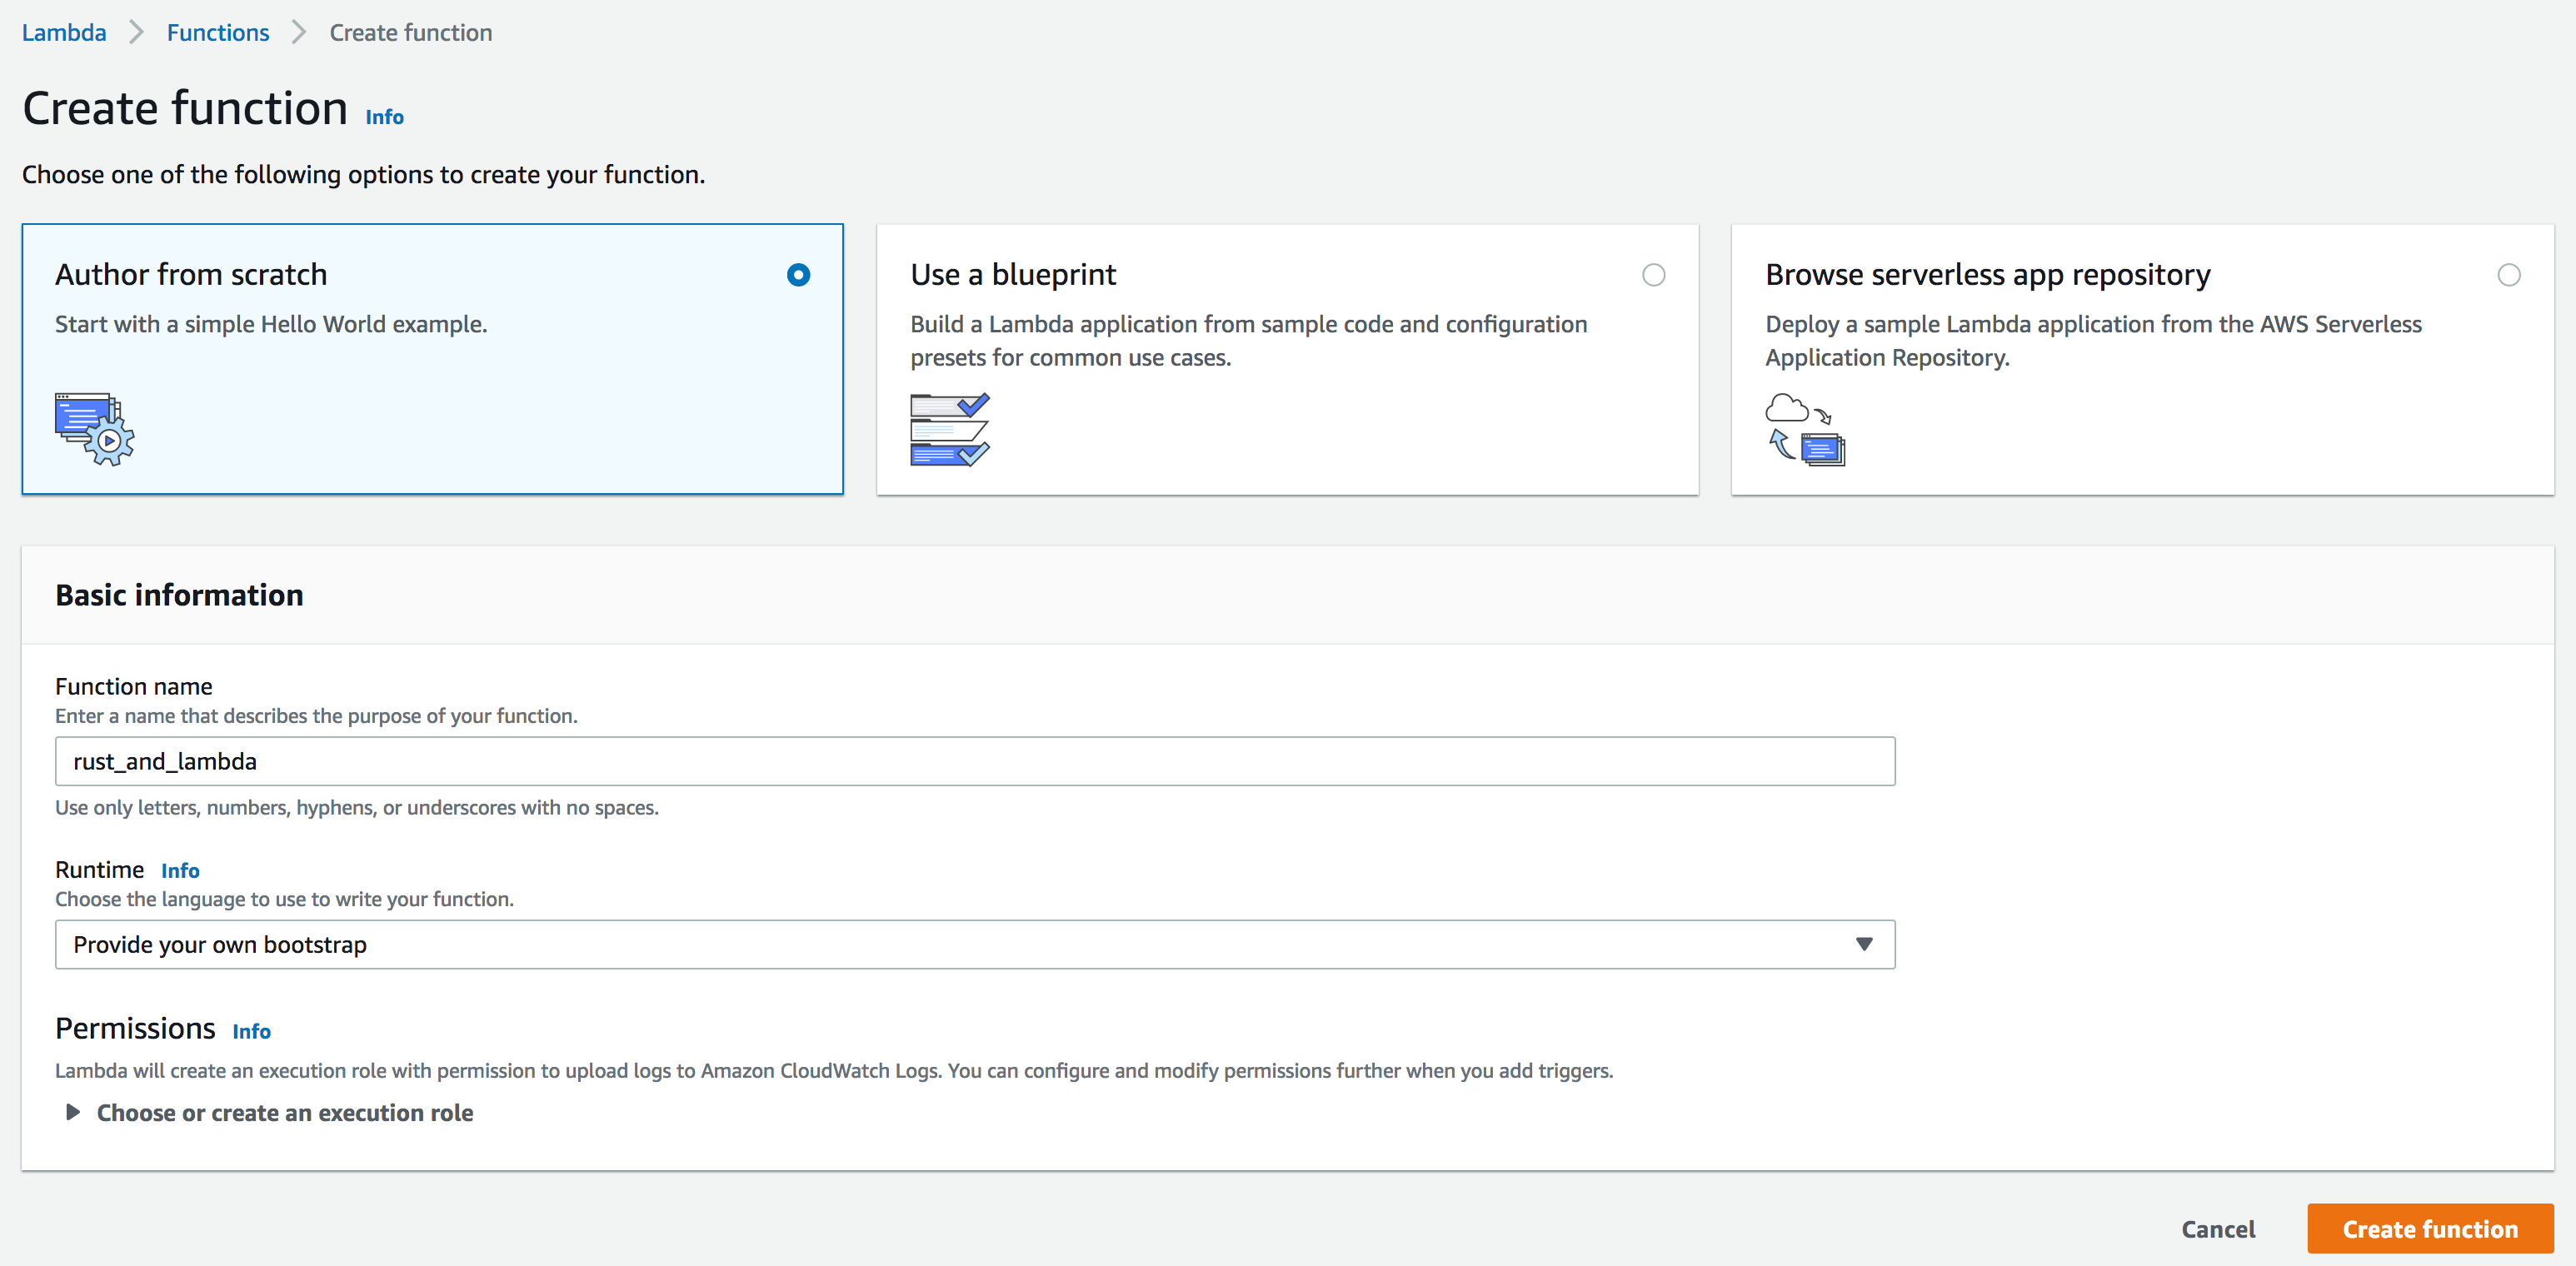
\includegraphics[width=0.8\linewidth]{lambda_create_function.png}
	\caption{Create lambda funcion}
	\label{fig:create_lambda_function}
\end{figure}

In the next page scroll below to function code. Click on code entry type and then select "Upload a .zip file". See Figure~\ref{fig:upload_method}

\begin{figure}[htpb]
	\centering
	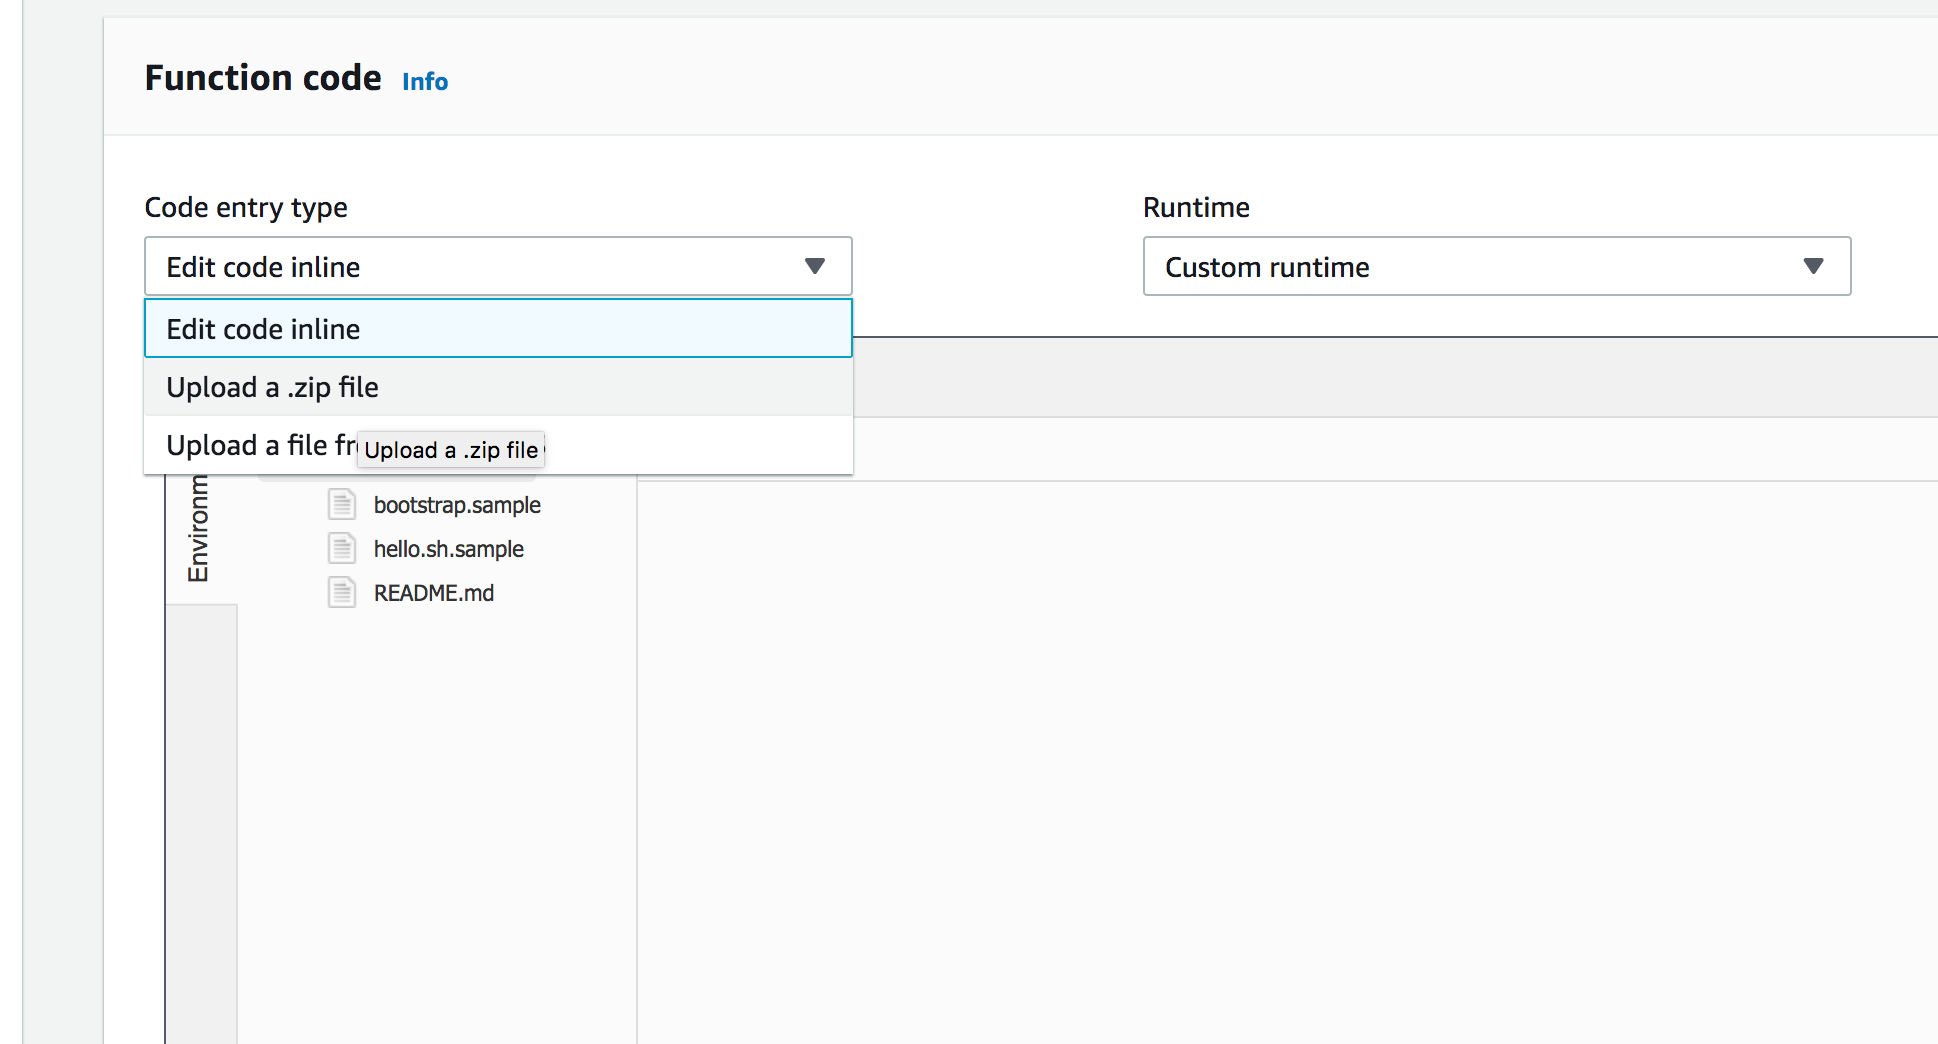
\includegraphics[width=0.8\linewidth]{select_upl_zip.png}
	\caption{select upload method}
	\label{fig:upload_method}
\end{figure}

Now we need to select the correct file and click the save button. This is shown in Figure~\ref{fig:select_zip_file}.

\begin{figure}[htpb]
	\centering
	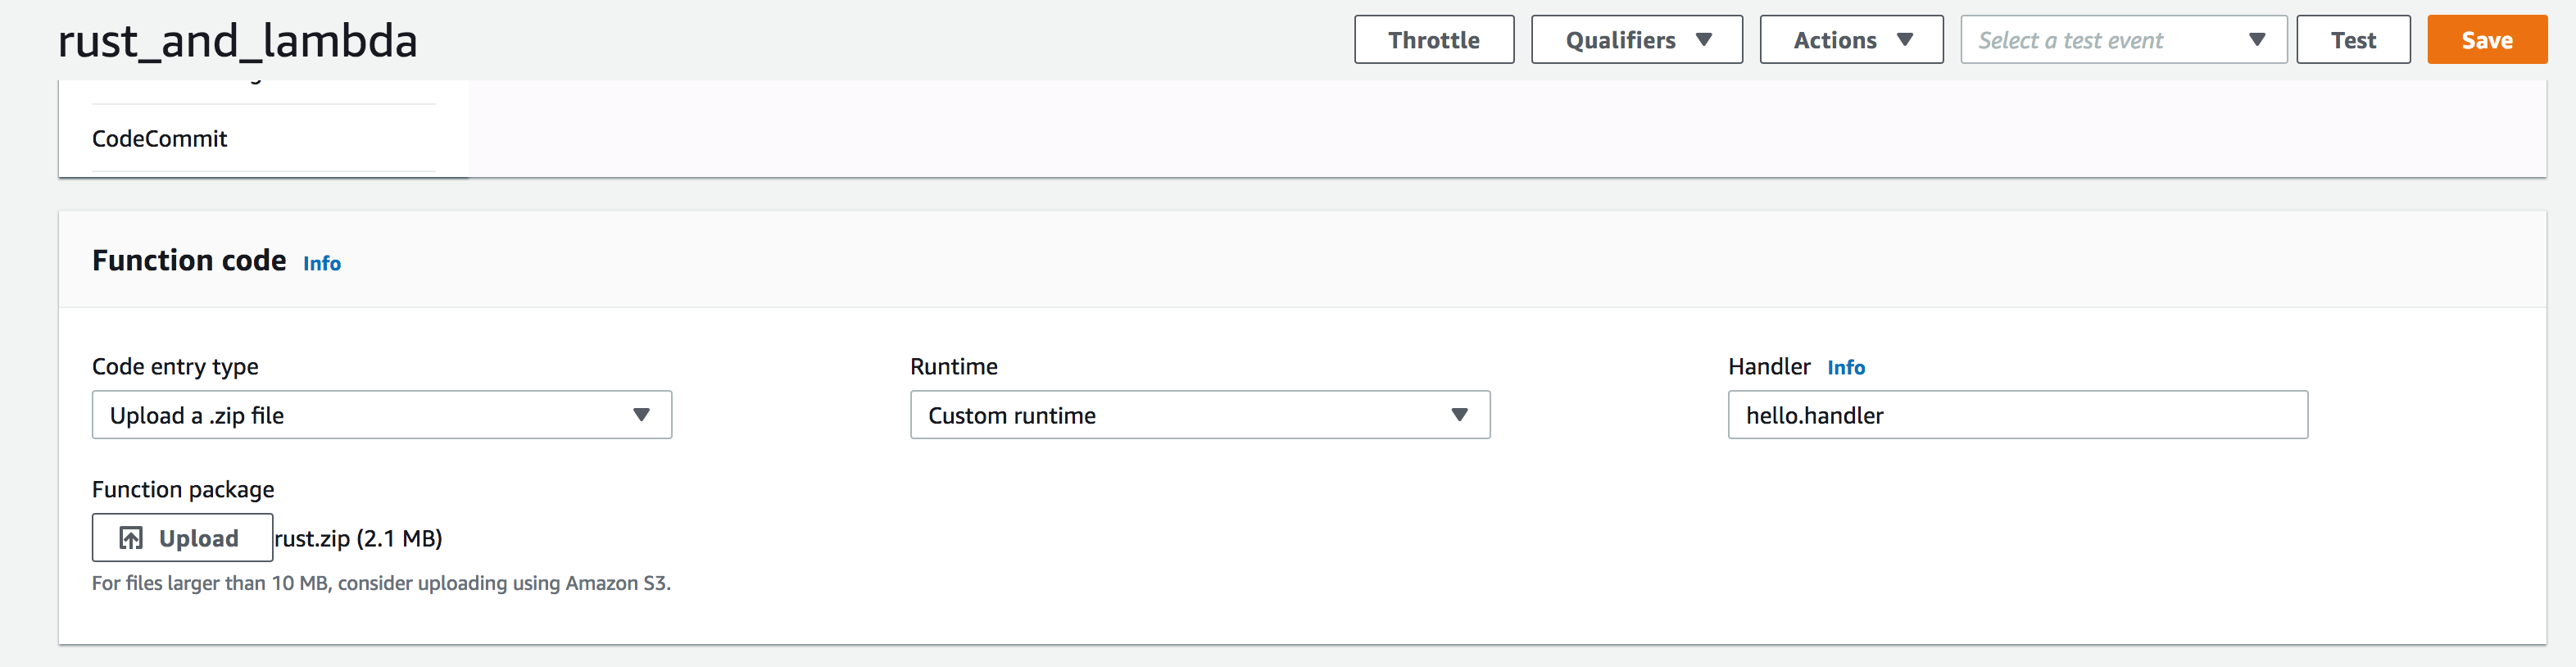
\includegraphics[width=0.8\linewidth]{select_file.png}
	\caption{select zip file}
	\label{fig:select_zip_file}
\end{figure}

Once saved our lambda function is created. We can now configure a test case in the console to see if the function is behaving as expected. This is shown in Figure~\ref{fig:test_case}. Since our function expects a string parameter we can pass a random sentence to the string parameter and that should give us the word count.

\begin{figure}[htpb]
	\centering
	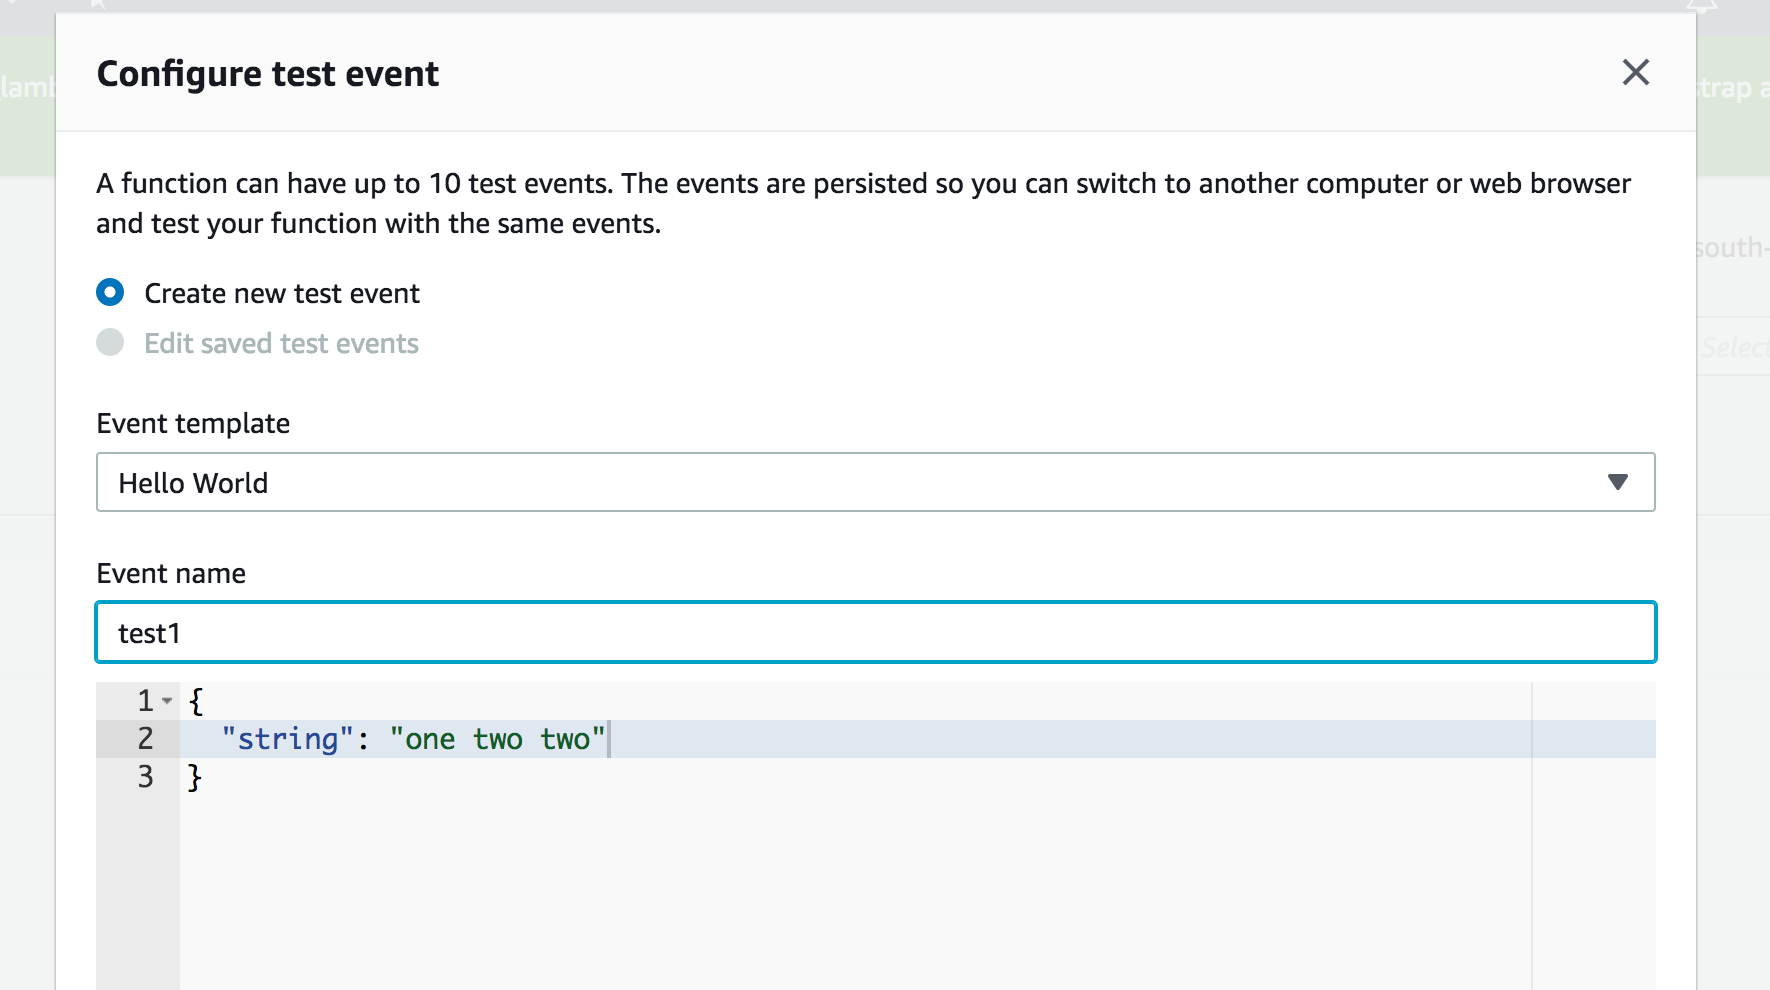
\includegraphics[width=0.5\linewidth]{test_case.png}
	\caption{test case}
	\label{fig:test_case}
\end{figure}

In Figure~\ref{fig:test_run} we see that running the test case gives us the correct result.

\begin{figure}[htpb]
	\centering
	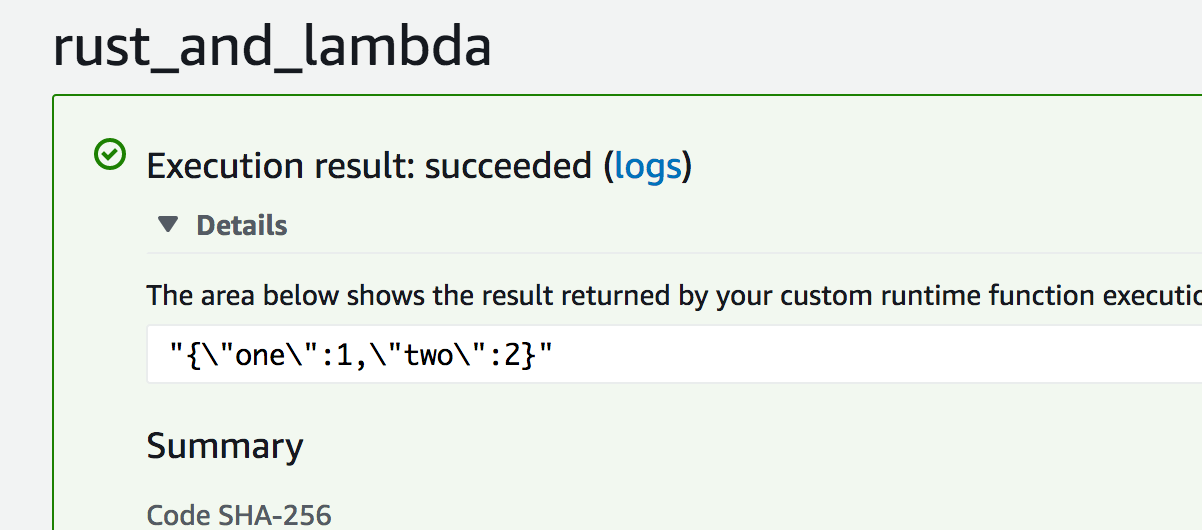
\includegraphics[width=0.5\linewidth]{run.png}
	\caption{test run}
	\label{fig:test_run}
\end{figure}

We have been successful in creating a serverless application in Rust. There are some caveats in this model of programming though. In our case the algorithm was simple and can be built easily using Rust. If the code is in pure Rust, the rust tooling that is built works and we should be able to build serverless applications easily. In case the applications have external library dependencies, such as the ones we have seen majorly in this book it is quite difficult to perform cross linking and compilation and create a binary for the AWS platform. Still if we are able to do that then model inference will work. Model training will work because that takes up time and serverless application have a timeout. In any case integrating serverless applications in the ML workflow gives in a huge productivity benefit to the developer.

\label{sec:rust_in_the_cloud}

\section{Conclusion}%

This last chapter introduced you to different ways in which Rust code can be integrated in an existing application. The chapter starts with writing wrappers for Python code using PyO3 and then we moved on to writing JNI wrapper code for using Rust code in Java. Finally we created a serverless application in AWS Lambda for an example for Rust in the cloud.

\label{sec:conclusion}

\printbibliography
\nocite{*}
\end{document}
